\documentclass[sigconf]{acmart}

\usepackage{booktabs}
\usepackage{graphicx}
\usepackage{tabularx}
\usepackage{tikz}
\usepackage{xurl}
\usetikzlibrary{arrows.meta,positioning}

\setcopyright{none}
\settopmatter{printacmref=false}
\renewcommand\footnotetextcopyrightpermission[1]{}
\pagestyle{plain}

\acmConference[ICNS3 2026]{International Conference on ns-3}{October 19--21, 2026}{Naples, Italy}
\acmYear{2026}
\copyrightyear{2026}

\title{From a Validation Example to a Reproducible TCP/AQM Benchmark in ns-3}

\author{Haoyu Wang}
\affiliation{%
  \department{Department of Computer Science}
  \institution{University of Massachusetts Boston}
  \city{Boston}
  \state{MA}
  \country{USA}}
\email{haoyu.wang001@umb.edu}

\author{Bo Sheng}
\affiliation{%
  \department{Department of Computer Science}
  \institution{University of Massachusetts Boston}
  \city{Boston}
  \state{MA}
  \country{USA}}
\email{bo.sheng@umb.edu}

\author{Xiaoqian Zhang}
\affiliation{%
  \department{College of Information Science \& Technology}
  \institution{University of Nebraska Omaha}
  \city{Omaha}
  \state{NE}
  \country{USA}}
\email{xiaoqianzhang@unomaha.edu}

% Short aliases keep artifact paths out of the prose; footnotes define paths.
\DeclareRobustCommand{\TcpAqmModule}{\textsc{ConfigMod}}
\DeclareRobustCommand{\TcpAqmBenchmark}{\textsc{BenchmarkEx}}
\DeclareRobustCommand{\TcpValidation}{\textsc{ValidationEx}}
\DeclareRobustCommand{\MetadataFile}{\textsc{RunMeta}}
\DeclareRobustCommand{\CommandFile}{\textsc{RunCmd}}
\DeclareRobustCommand{\StdoutFile}{\textsc{StdoutLog}}
\DeclareRobustCommand{\StderrFile}{\textsc{StderrLog}}
\DeclareRobustCommand{\ConfigJson}{\textsc{RunConfig}}
\DeclareRobustCommand{\TraceGlob}{\textsc{TraceSet}}
\DeclareRobustCommand{\SummaryCsv}{\textsc{RunSummary}}
\DeclareRobustCommand{\SummaryAggregateCsv}{\textsc{AggregateSummary}}
\DeclareRobustCommand{\FullSummaryCsv}{\textsc{SingleFlowRows}}
\DeclareRobustCommand{\FullSummaryAggregateCsv}{\textsc{SingleFlowAgg}}
\DeclareRobustCommand{\MixedSummaryCsv}{\textsc{MixedFlowRows}}
\DeclareRobustCommand{\MixedSummaryAggregateCsv}{\textsc{MixedFlowAgg}}
\DeclareRobustCommand{\DataDir}{\textsc{DataSet}}
\DeclareRobustCommand{\CoreEvalDir}{\textsc{CoreEvalData}}
\DeclareRobustCommand{\PaperFigureDir}{\textsc{CoreEvalFigs}}
\DeclareRobustCommand{\RsvgConvert}{\texttt{rsvg-convert}}
\DeclareRobustCommand{\Latexmk}{\texttt{latexmk}}
\DeclareRobustCommand{\MainTex}{\textsc{MainSource}}
\newcommand{\CodeArtifactPaths}{\footnote{\TcpAqmModule{} denotes \path{contrib/tcp-aqm-config/}; \TcpAqmBenchmark{} denotes \path{contrib/tcp-aqm-config/examples/tcp-aqm-benchmark.cc}; \TcpValidation{} denotes \path{examples/tcp/tcp-validation.cc}.}}
\newcommand{\RunArtifactPaths}{\footnote{\MetadataFile{} denotes \path{metadata.json}; \CommandFile{} denotes \path{command.txt}; \StdoutFile{} denotes \path{stdout.txt}; \StderrFile{} denotes \path{stderr.txt}; \ConfigJson{} denotes \path{config.json}; \TraceGlob{} denotes \path{tcp-aqm-benchmark-*.dat}; \SummaryCsv{} denotes \path{summary.csv}; \SummaryAggregateCsv{} denotes \path{summary-aggregate.csv}.}}
\newcommand{\PaperArtifactPaths}{\footnote{\FullSummaryCsv{} denotes \path{data/full-summary.csv}; \FullSummaryAggregateCsv{} denotes \path{data/full-summary-aggregate.csv}; \MixedSummaryCsv{} denotes \path{data/mixed-summary.csv}; \MixedSummaryAggregateCsv{} denotes \path{data/mixed-summary-aggregate.csv}; \DataDir{} denotes \path{data/}; \CoreEvalDir{} denotes \path{data/core-eval/}; \PaperFigureDir{} denotes \path{fig/tcp-aqm/core-eval/}; \MainTex{} denotes \path{main.tex}.}}
\newcommand{\RttSensitivityFigure}{fig/tcp-aqm/core-eval/rtt-throughput-sensitivity.pdf}
\newcommand{\MixedShareFigure}{fig/tcp-aqm/core-eval/mixed-flow-share.pdf}
\newcommand{\WarmupSensitivityFigure}{fig/tcp-aqm/core-eval/warmup-sensitivity.pdf}

\begin{document}

\begin{abstract}
Comparing TCP congestion control and active queue management in ns-3 is highly sensitive to topology, RTT, ECN configuration, queue discipline defaults, flow mix, and random seeds, yet many simulation studies report only a handful of manually executed scenarios. This paper presents a reproducible ns-3 benchmark workflow for TCP/AQM studies and demonstrates it through baseline single-flow and mixed-flow comparisons of Linux Reno, CUBIC, and DCTCP with CoDel, FQ-CoDel, PIE, and RED. The workflow ships as a small contrib module that loads YAML or JSON experiment and topology descriptions, expands matrices over seeded random-run values, and preserves command lines, environment metadata, and raw traces per run alongside summary tables and vector figures. The benchmark scenario is derived from the in-tree TCP validation example, inheriting a known-good dumbbell topology and validation cases without modifying the upstream example. The case study reports throughput, fairness, RTT, queueing delay, drops, and ECN marks across base RTT, ECN, and competing-flow settings, distinguishing conclusions that hold across configurations from those that depend on specific assumptions. The artifact is designed to be rerun, audited, and extended by ns-3 users, and is available on the \texttt{icns3-summer-2026-benchmark} branch of our ns-3 fork.\footnote{\url{https://github.com/Haoyu2/ns3/tree/icns3-summer-2026-benchmark}}

\end{abstract}

\begin{CCSXML}
<ccs2012>
 <concept>
  <concept_id>10003033.10003039.10003041</concept_id>
  <concept_desc>Networks~Network simulations</concept_desc>
  <concept_significance>500</concept_significance>
 </concept>
 <concept>
  <concept_id>10003033.10003079.10003080</concept_id>
  <concept_desc>Networks~Transport protocols</concept_desc>
  <concept_significance>500</concept_significance>
 </concept>
</ccs2012>
\end{CCSXML}

\ccsdesc[500]{Networks~Network simulations}
\ccsdesc[500]{Networks~Transport protocols}

\keywords{ns-3, TCP, active queue management, ECN, reproducibility, congestion control}

\maketitle

\section{Introduction}

ns-3 is widely used to evaluate transport protocols and queue-management mechanisms, but TCP/AQM simulation results can be difficult to compare across papers. A conclusion such as ``queue discipline X improves delay'' or ``congestion control Y better utilizes the bottleneck'' depends on details that are easy to omit: the base RTT, queue-disc defaults, ECN configuration, traffic start time, random-run value, trace-processing method, and warmup interval. When those details are not preserved as runnable artifacts, reproducing or extending a study becomes unnecessarily fragile.

This paper focuses on TCP/AQM evaluation as an ns-3 methodology problem. Rather than proposing a new congestion-control algorithm, we contribute a reproducible benchmark workflow and use it to generate baseline results over ns-3's existing TCP and traffic-control models. The workflow records exact command lines, ns-3 commit metadata, run parameters, raw traces, and derived summary statistics. It also introduces \TcpAqmModule{}, a small C++ contrib configuration module that reads YAML or JSON experiment and topology descriptions.\CodeArtifactPaths{} The benchmark remains intentionally lightweight: it derives a module example from the in-tree \TcpValidation{} scenario so that researchers can reuse a known topology without changing the original validation example.

The case study compares TCP Linux Reno, CUBIC, and DCTCP across CoDel, FQ-CoDel, PIE, and RED. We vary base RTT and ECN support in the single-flow campaign, then add a mixed-flow campaign with competing TCP pairs and randomized second-flow start times. The reported metrics include throughput, fairness, RTT, bottleneck queueing delay, congestion window behavior, drops, and ECN marks. The goal is not to declare a universal winner among queue disciplines. Instead, the goal is to show which conclusions are stable, which depend on experimental assumptions, and how ns-3 users can package TCP/AQM studies so that others can rerun them.

This paper makes five contributions:

\begin{enumerate}
  \item A reproducible TCP/AQM benchmark harness for ns-3, implemented as \TcpAqmBenchmark{} and derived from the validated \TcpValidation{} topology.
  \item A C++ contrib configuration module that loads YAML/JSON experiment and topology descriptions and provides single-bottleneck and two-bottleneck templates.
  \item A traceable artifact structure that preserves command lines, random-run values, raw traces, stdout/stderr, and git metadata.
  \item Baseline single-flow and mixed-flow comparisons of TCP congestion-control and AQM interactions under multiple RTT, ECN, queue-discipline, and flow-mix settings.
  \item Practical reporting recommendations for future ns-3 TCP/AQM studies.
\end{enumerate}

\section{Background and Motivation}

The ns-3 TCP model includes multiple congestion-control algorithms, including Linux Reno, CUBIC, DCTCP, and BBR. This capability builds on a substantial redesign of ns-3 TCP architecture and later model contributions for both loss-based and model-based congestion control~\cite{Casoni2016NextGenerationTcp,Nguyen2016TcpVariants,Jain2018Bbr}. The traffic-control module introduces a Linux-like queue-disc layer in ns-3, enabling studies of CoDel, FQ-CoDel, PIE, RED, and related variants~\cite{Imputato2016TrafficControl,Shravya2016Pie}. These models make ns-3 a natural platform for transport and queue-management studies, but they also introduce a large configuration space.

TCP/AQM comparisons are particularly sensitive to hidden assumptions. ECN-enabled queues change whether congestion is signaled by marking or dropping. RTT changes the time required for a flow to reach steady state. Queue-disc defaults affect target delay, marking thresholds, and drop behavior. Some queue disciplines include randomness, so single-run results may overstate a conclusion. These sensitivities are not flaws in ns-3; they are reasons to make experiment design explicit and reproducible.

The starting point for this work is the in-tree TCP validation program. That example provides a dumbbell topology, single-flow and optional second-flow TCP traffic, ping RTT measurement, bottleneck queue tracing, and validation cases for selected CUBIC and DCTCP behavior. Our benchmark preserves that topology as an anchor but moves paper-specific generalization into a new example so the original validation example remains unchanged.

\section{Related Work and Positioning}

This work builds on two strands of ns-3 research: model implementation and evaluation infrastructure. The modern ns-3 TCP architecture separates congestion-control behavior from the socket machinery, making it practical to compare TCP variants within a common simulator framework~\cite{Casoni2016NextGenerationTcp}. The traffic-control module similarly provides the queue-disc abstraction used by CoDel, FQ-CoDel, PIE, RED, and related AQM studies~\cite{Imputato2016TrafficControl}. Prior WNS3 work has also added or validated individual transport and AQM models, including PIE, additional TCP congestion controls, and TCP BBR~\cite{Shravya2016Pie,Nguyen2016TcpVariants,Jain2018Bbr}. Our benchmark does not contribute a new TCP or queue-disc model; it packages existing models into a reproducible TCP/AQM interaction study.

The ns-3 community has also produced substantial evaluation infrastructure for transport and queue-management studies. Mishra, Vankar, and Tahiliani introduced a TCP Evaluation Suite for ns-3 based on ICCRG evaluation guidance, automating simulation setup, topology creation, traffic generation, execution, and result collection for several TCP extensions and scenarios, including bandwidth, RTT, bottleneck, and long-flow-count variation~\cite{Mishra2016TcpEval}. Nagori et al. later presented a Common TCP Evaluation Suite for ns-3 that integrates Tmix realistic TCP traffic and validates its behavior against an ns-2 implementation, while also reporting open issues in the integration~\cite{Nagori2017CommonTcpEval}.

AQM evaluation has also been addressed directly. Deepak, Shravya, and Tahiliani presented an AQM Evaluation Suite for ns-3 aligned with RFC 7928, automating topology construction, traffic generation, execution, result collection, and graphical output for AQM studies~\cite{Deepak2017AqmEval,Kuhn2016Rfc7928}. More recently, the AQM Evaluation Suite has been modernized for ns-3.45, CMake, newer AQM and ECN functionality, and ns-3 App Store packaging~\cite{Ns3AppStore2025AqmEval,Lin2025GSoCAqmEval}.

Accordingly, this paper is not positioned as the first TCP or AQM evaluation suite for ns-3. The contribution is deliberately narrower and artifact-oriented: we study how an in-tree, validated TCP example in current ns-3 can be turned into a lightweight benchmark artifact for TCP/AQM interaction studies. The benchmark uses ns-3's TCP validation example as an anchor but packages the paper artifact as \TcpAqmBenchmark{} in \TcpAqmModule{}, preserving raw traces and exact command provenance while examining whether TCP/AQM conclusions remain stable as RTT, ECN, queue discipline, flow mix, and random-run values change.

\begin{table}[t]
  \caption{Positioning relative to closest ns-3 TCP/AQM evaluation work.}
  \label{tab:related-positioning}
  \begin{tabularx}{\columnwidth}{@{}p{0.31\columnwidth}X@{}}
    \toprule
    Prior work & Relationship to this paper \\
    \midrule
    TCP Evaluation Suite~\cite{Mishra2016TcpEval} & Broad ICCRG-style TCP evaluation automation. Our artifact is narrower and focuses on current TCP/AQM interaction traceability. \\
    Common TCP Evaluation Suite~\cite{Nagori2017CommonTcpEval} & Tmix traffic and ns-2 validation. Our work does not replace realistic traffic generation; it provides a lightweight audited benchmark. \\
    AQM Evaluation Suite~\cite{Deepak2017AqmEval} & RFC 7928-aligned AQM automation. Our work studies the intersection of TCP variant, AQM, ECN, RTT, and seeds. \\
    AQM Suite upgrade~\cite{Ns3AppStore2025AqmEval,Lin2025GSoCAqmEval} & Modernized broad AQM suite. Our artifact is intentionally smaller and derived from an in-tree validation example. \\
    This paper & Lightweight current-ns-3 benchmark derived from \TcpValidation{} and packaged in \TcpAqmModule{}; emphasizes YAML/JSON configuration, raw trace preservation, provenance, and TCP/AQM sensitivity across RTT, ECN, flow mix, and seeds. \\
    \bottomrule
  \end{tabularx}
\end{table}

\section{Benchmark Design}

The benchmark uses the dumbbell topology from \TcpValidation{} as its validation anchor, with the paper-specific scenario implemented as \TcpAqmBenchmark{}. Servers connect through a WAN router to one or more bottleneck links, then through a LAN router to clients. TCP data flows traverse the bottleneck path in the downstream direction, and a ping flow measures RTT. The bottleneck queue discipline is selected at runtime.

The current implementation keeps benchmark configuration and the runnable scenario together inside a small contrib module, \TcpAqmModule{}. The module provides C++ experiment and topology configuration objects and reads YAML or JSON files using \texttt{yaml-cpp}. This lets the same benchmark binary run from either command-line arguments or versioned configuration files. The first topology templates are intentionally constrained: a single bottleneck and two serial bottlenecks. This keeps the artifact reviewable while showing how topology structure can be externalized without editing the scenario source.

The primary experiment matrix in this paper varies three of the seventeen TCP TypeIds the module accepts:

\begin{itemize}
  \item TCP variant: Linux Reno, CUBIC, DCTCP (selected from the seventeen TCP TypeIds the module accepts, including BBR, NewReno, Vegas, Veno, YeAH, BIC, Westwood+, Illinois, HighSpeed, Hybla, H-TCP, Scalable, LEDBAT, and LP).
  \item Queue discipline: CoDel, FQ-CoDel, PIE, RED.
  \item Base RTT: 10 ms, 50 ms, 80 ms.
  \item ECN: disabled or enabled at the bottleneck queue.
  \item Random run: one or more \texttt{RngRun} values.
  \item Flow mix: a single TCP flow or a configured pair of competing flows.
\end{itemize}

Configuration files record the same factors, plus topology-specific values such as access-link rate, access-link delay, device queue size, bottleneck rates, bottleneck delays, which bottleneck queue is traced, and flow timing parameters. When bottleneck delays are omitted, the C++ configuration object derives one-way delays from the requested base RTT. For mixed-flow runs, the second flow can start from a configured base time plus a bounded jitter that is driven by \texttt{RngRun}, making the stochastic element explicit in the artifact. The two-bottleneck template is presently used only as a smoke-path scenario; all paper-reported results use the single-bottleneck template, and the two-bottleneck campaign is left as future work.

The same harness can run additional TCP TypeIds, such as BBR, but those results should be reported as an extension unless the campaign includes enough repetitions and discussion to interpret model-based pacing behavior fairly.

The primary metrics are mean throughput, ping RTT, bottleneck queueing delay, congestion window, packet drops, and ECN marks after a warmup interval. Raw traces are retained so that additional metrics can be computed without rerunning simulations.

\section{Workflow Implementation}

The workflow consists of \TcpAqmModule{}, \TcpAqmBenchmark{}, and Python runner and analysis scripts. The contrib module defines typed C++ objects for experiment and topology configuration. These objects load YAML or JSON files through \texttt{yaml-cpp}, validate the experiment and topology sections, map TCP and queue-disc names into enum values, store scalar values as ns-3 \texttt{Time}, \texttt{DataRate}, and \texttt{QueueSize} objects, and derive omitted bottleneck delays from the configured base RTT.

The C++ benchmark example resolves TCP aliases and TypeId names, configures the selected TCP variants per node, and keeps DCTCP-specific alpha tracing attached only when the resolved TypeId is DCTCP. This lets a campaign use short names such as \texttt{cubic} and \texttt{dctcp}, or full names such as \texttt{ns3::TcpBbr}, without changing the scenario source. The same binary can also be launched with \texttt{--configFile}, allowing a versioned configuration file to select a single-bottleneck or two-bottleneck topology and to control flow start times. For mixed-flow runs, the second flow can receive a bounded start-time jitter that is driven by the configured ns-3 random-run value.

The runner expands a named experiment matrix and invokes \texttt{./ns3 run} for each configuration. Each run receives an explicit \texttt{rngRun} value and stores a compact set of run artifacts:\RunArtifactPaths{}

\begin{itemize}
  \item Run metadata in \MetadataFile{}, including parameters, ns-3 commit, branch state, working-tree status, SHA-256 hashes of every benchmark and configuration source file that contributed to the run, a snapshot of ns-3-relevant environment variables (\texttt{NS\_LOG}, \texttt{NS\_GLOBAL\_VALUE}, \texttt{LD\_LIBRARY\_PATH}, and similar), return code, resolved trace files, and wall-clock time.
  \item \CommandFile{}, containing the exact ns-3 command.
  \item \StdoutFile{} and \StderrFile{}.
  \item Raw \TraceGlob{} trace files.
\end{itemize}

When the working tree contains modifications to the benchmark example, the contrib module sources, or any configuration file referenced by the run, the runner prints a warning. The per-file SHA-256 hashes still pin the exact source bytes used by that run, so a dirty tree does not silently invalidate the artifact.

The analyzer reads each run directory and writes a campaign-level \SummaryCsv{} and \SummaryAggregateCsv{}. The summaries include throughput, RTT, queueing delay, congestion window, drop count, mark count, and, for mixed-flow runs, second-flow throughput, total throughput, and Jain fairness (defined for the two-flow case used in this study). The analyzer clamps a configured warmup threshold below the first-flow start time so that pre-flow zero samples cannot deflate mean throughput. A dependency-free SVG plotter creates quick figures from the aggregate table for inspection before final plotting.

The contrib module includes a validation executable that loads a YAML or JSON file and prints the normalized configuration. This provides a lightweight check that configuration files are syntactically valid, semantically complete, and produce the intended derived topology values before a campaign is launched.

\begin{figure}[t]
  \centering
  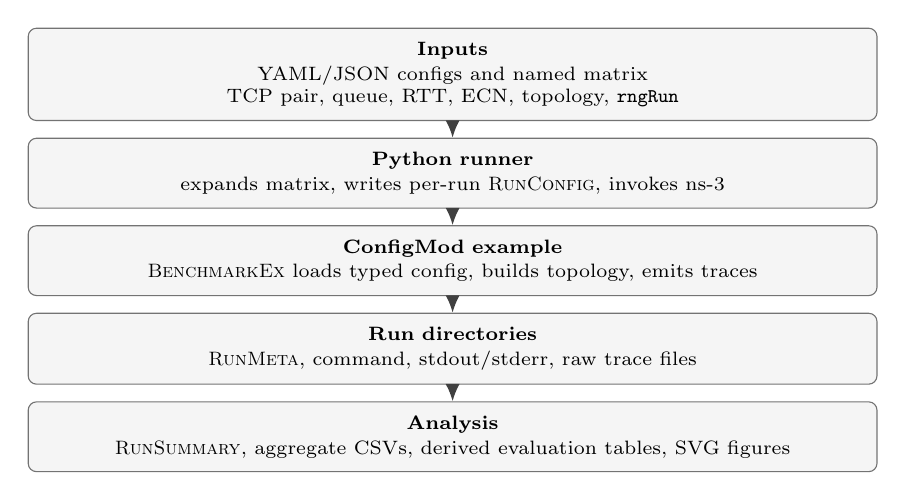
\begin{tikzpicture}[
    node distance=0.6em and 0.6em,
    stage/.style={
      draw=black!55,
      line width=0.4pt,
      fill=black!4,
      rounded corners=3pt,
      align=center,
      text width=0.86\columnwidth,
      inner sep=5pt,
      font=\scriptsize,
    },
    header/.style={font=\scriptsize\bfseries},
    arrow/.style={
      -{Latex[length=2.2mm,width=1.8mm]},
      line width=0.7pt,
      draw=black!75,
    },
  ]
    \node[stage] (config) {%
      \textbf{Inputs}\\[1pt]
      YAML/JSON configs and named matrix\\
      \scriptsize TCP pair, queue, RTT, ECN, topology, \texttt{rngRun}};
    \node[stage, below=of config] (runner) {%
      \textbf{Python runner}\\[1pt]
      expands matrix, writes per-run \ConfigJson{}, invokes ns-3};
    \node[stage, below=of runner] (ns3) {%
      \textbf{\TcpAqmModule{} example}\\[1pt]
      \TcpAqmBenchmark{} loads typed config, builds topology, emits traces};
    \node[stage, below=of ns3] (runs) {%
      \textbf{Run directories}\\[1pt]
      \MetadataFile{}, command, stdout/stderr, raw trace files};
    \node[stage, below=of runs] (analysis) {%
      \textbf{Analysis}\\[1pt]
      \SummaryCsv{}, aggregate CSVs, derived evaluation tables, SVG figures};
    \draw[arrow] (config) -- (runner);
    \draw[arrow] (runner) -- (ns3);
    \draw[arrow] (ns3) -- (runs);
    \draw[arrow] (runs) -- (analysis);
  \end{tikzpicture}
  \caption{Reproducible TCP/AQM benchmark workflow. Each stage's output is the input of the stage below.}
  \Description{Vertical workflow diagram with five stages: inputs, Python runner, ns-3 benchmark example, run directories, and analysis; each stage is connected to the next by a downward arrow.}
  \label{fig:workflow}
\end{figure}

\section{Evaluation Results}

The current evaluation is artifact-first: every plotted result is derived from a preserved CSV table, and each table can be traced back to per-run metadata and raw ns-3 traces. The pilot campaign contains 180 successful single-flow runs and 36 successful mixed-flow runs, with zero failed return codes. These runs expose the main sensitivity patterns and identify which configurations need a longer final timing campaign.

\begin{table}[t]
  \caption{Validated single-flow campaign. DCTCP without ECN is excluded from the main comparison.}
  \label{tab:matrix}
  \centering
  \small
  \begin{tabular}{@{}ll@{}}
    \toprule
    Factor & Values \\
    \midrule
    TCP & Linux Reno, CUBIC, DCTCP \\
    Queue discipline & CoDel, FQ-CoDel, PIE, RED \\
    Base RTT & 10, 50, 80 ms \\
    ECN & off/on (DCTCP requires on) \\
    Seeds & 3 \texttt{RngRun} values \\
    Stop / warmup & 40 s / 10 s \\
    Rows (per-run / aggregate) & 180 / 60 \\
    \bottomrule
  \end{tabular}
\end{table}

\subsection{Single-Flow Throughput Dispersion Across RTT}

Figure~\ref{fig:rtt-sensitivity} summarizes how each ECN-enabled single-flow configuration's mean throughput disperses across base RTT, reported as $100\cdot(\max-\min)/\max$ over the three RTT means. We use the term \emph{dispersion} rather than \emph{sensitivity} to avoid implying a monotone response: this metric measures spread, not signed slope. PIE produces the widest dispersion in this pilot matrix: DCTCP/PIE varies by 51.6\% of its maximum throughput across 10, 50, and 80 ms, while Reno/PIE and CUBIC/PIE vary by about 32\%. DCTCP with CoDel and FQ-CoDel also varies by about 31\%, showing that low-delay behavior does not automatically imply RTT-insensitive throughput.

\begin{figure*}[t]
  \centering
  \includegraphics[width=0.84\textwidth]{\RttSensitivityFigure}
  \caption{Single-flow throughput dispersion across 10, 50, and 80 ms base RTT for ECN-enabled configurations. Bars are $100\cdot(\max-\min)/\max$ of mean throughput across the three RTT settings; this measures spread, not signed slope.}
  \Description{Horizontal bar chart ranking ECN-enabled TCP and queue configurations by throughput dispersion across base RTT values.}
  \label{fig:rtt-sensitivity}
\end{figure*}

The full single-flow throughput/delay scatter and Pareto-frontier table are archived with the artifact. They show why a single ranking is misleading: CUBIC often remains near the throughput frontier, while DCTCP can occupy low-delay points with lower throughput at high RTT. RED and CoDel appear frequently on the non-dominated frontier in this pilot, while PIE appears only once. Single-flow aggregate confidence intervals are not reported here because the pilot campaign drove no stochastic input in the single-flow scenario; the three \texttt{RngRun} values produce numerically identical traces, so the corresponding 95\% confidence intervals are structurally zero rather than tight. The harness records the per-run \texttt{rngRun} value regardless, and future single-flow campaigns can produce meaningful confidence intervals by sweeping the existing \texttt{firstStartTime} field or by enabling the new \texttt{firstStartJitter} input.

\subsection{Mixed-Flow Behavior}

The mixed-flow campaign uses three TCP pairs, CoDel and FQ-CoDel, 10 ms and 80 ms base RTT, ECN enabled, and three \texttt{RngRun} values. The second flow starts at 10 s plus up to 5 s of random-run-driven jitter, the stop time is 40 s, and the analysis discards the first 20 s. This campaign produced 36 successful runs and 12 aggregate rows.

Figure~\ref{fig:mixed-share} shows that total bottleneck utilization can hide large per-flow asymmetry. At 10 ms, DCTCP receives 95.8\% of total throughput when paired with CUBIC under CoDel and 88.3\% when paired with Reno. FQ-CoDel improves the CUBIC/Reno pair most strongly: the 10 ms fairness score rises from 0.733 to 0.9998 with essentially unchanged total throughput. The FQ-CoDel fairness-delta chart and the complete mixed-flow table are archived in \CoreEvalDir{} and \PaperFigureDir{}.

\begin{figure*}[t]
  \centering
  \includegraphics[width=0.88\textwidth]{\MixedShareFigure}
  \caption{Mixed-flow throughput share by TCP pair, queue discipline, and base RTT. The right column reports total throughput and Jain fairness.}
  \Description{Stacked horizontal bar chart showing first-flow and second-flow throughput share for each mixed TCP pair.}
  \label{fig:mixed-share}
\end{figure*}

\subsection{Warmup and Stability Audits}

The analysis pipeline also recomputes each campaign under multiple warmup thresholds and compares the final quarter of each run against the preceding quarter. These audits are not a separate networking claim; they are a reproducibility check on whether the current 40 s pilot campaign is long enough for final performance conclusions.

Figure~\ref{fig:warmup} shows that 32 of 72 aggregate configurations have more than 5\% throughput range across the tested warmups. The chart is grouped by campaign so both single-flow and mixed-flow are always represented: the top 12 single-flow rows out of 60, and the top 6 mixed-flow rows out of 12. The largest-warmup threshold in the sweep (30 s, paired with a 40 s stop time) leaves only ten seconds of measurement window and should be read as a stress test, not as a recommended operating point. The late-window audit similarly flags 97 of 252 observations with more than 5\% difference between the final quarter and the preceding quarter, with the largest deviations appearing in high-RTT DCTCP/PIE and selected mixed-flow cases. This converts a vague concern about transient behavior into a concrete next-step requirement: the final artifact should include a longer targeted campaign for the unstable configurations.

\begin{figure*}[t]
  \centering
  \includegraphics[width=0.86\textwidth]{\WarmupSensitivityFigure}
  \caption{Warmup-sensitivity audit, grouped by campaign. Bars show the throughput range across tested warmup thresholds (5, 10, 20, 30 s for single-flow; 15, 20, 25, 30 s for mixed-flow) as a percentage of the maximum observed value. The chart shows the top 12 single-flow rows out of 60 and the top 6 mixed-flow rows out of 12; the full table is archived with the artifact.}
  \Description{Two-group horizontal bar chart: top 12 single-flow configurations and top 6 mixed-flow configurations ranked by throughput variation across warmup thresholds.}
  \label{fig:warmup}
\end{figure*}

The full single-flow aggregate table, mixed-flow aggregate table, derived audit CSVs, and additional vector figures are archived under \DataDir{} and \PaperFigureDir{}.

\section{Discussion}

The completed campaigns illustrate a central methodological point: stop time, warmup interval, RTT, queue-disc settings, and flow mix jointly shape the interpretation of TCP/AQM results. The earlier smoke run was adequate for checking that the workflow executed, but it under-represented high-RTT behavior. The full campaign therefore makes the stop time and warmup interval explicit and stores them with every run.

The benchmark also makes ECN configuration explicit at both the TCP and queue-disc layers. DCTCP is excluded from the main non-ECN comparison because DCTCP without queue marking is not a meaningful protocol comparison. Such cases can still be useful as warnings or failure-mode checks, but they should not be mixed into the main result matrix.

The full single-flow campaign also reveals a limitation of deterministic traffic. Three random-run values are useful for reproducibility bookkeeping, but they do not create meaningful variability when the scenario does not consume random variables. In the present single-flow campaign, the three \texttt{RngRun} values produce numerically identical traces because no stochastic input is sampled; reported single-flow confidence intervals are therefore structurally zero, not tight, and we choose to disclose this rather than display them. The mixed-flow campaign addresses this by adding a competing flow and \texttt{rngRun}-driven start jitter. The resulting mixed-flow confidence intervals do reflect controlled workload variation. The harness has since been extended with a first-flow \texttt{firstStartJitter} input so that future single-flow campaigns can produce equally meaningful confidence intervals without changing scenario semantics.

The ECN comparison is a useful negative result in the current pilot. For single-flow CUBIC and Reno, enabling ECN changes mean queueing delay by only a small amount under many configurations, while DCTCP depends on ECN marking and is therefore treated separately. This does not mean ECN is unimportant; it means the paper should avoid over-claiming from a single-flow deterministic topology and should emphasize the interaction between TCP semantics, queue marking, and workload mix.

The warmup and late-window audits also change how the final evaluation should be framed. Several 40 s configurations, especially high-RTT DCTCP/PIE and selected mixed-flow cases, do not appear stable enough for final performance claims. Rather than hiding this, the artifact exposes it. The next campaign should therefore be targeted: rerun the unstable configurations with longer stop times and report whether rankings and fairness conclusions survive the longer observation window.

Finally, preserving raw traces changes the reviewability of the experiment. Throughput summaries alone can hide queueing-delay behavior, and aggregate means can hide transient or tail behavior. Keeping raw queue length, mark, drop, RTT, throughput, and congestion-window traces allows later analyses to be added without rerunning the full campaign.

\section{Artifact and Reproducibility}

The artifact is organized so each run can be traced back to an exact command, parameter set, random-run value, and ns-3 commit. The runnable benchmark is \TcpAqmBenchmark{}; the upstream validation anchor, \TcpValidation{}, remains unchanged. A typical run directory contains \MetadataFile{}, \CommandFile{}, \StdoutFile{}, \StderrFile{}, and raw \TraceGlob{} traces.

The paper repository archives the CSVs and figures used in this draft. Single-flow summaries are stored as \FullSummaryCsv{} and \FullSummaryAggregateCsv{}; mixed-flow summaries are stored as \MixedSummaryCsv{} and \MixedSummaryAggregateCsv{}. Derived evaluation tables are under \CoreEvalDir{}. The SVG sources and paper-facing PDF figures are under \PaperFigureDir{}.\PaperArtifactPaths{}

\begin{table}[t]
  \caption{Artifact commands and outputs. Exact command lines are preserved in the artifact README and per-run metadata.}
  \label{tab:artifact-commands}
  \centering
  \small
  \begin{tabularx}{\columnwidth}{@{}lX@{}}
    \toprule
    Step & Command family / output \\
    \midrule
    Single-flow campaign & Runner script in single-flow mode; analyzer uses a 10 s warmup. \\
    Mixed-flow campaign & Runner script in mixed-flow mode; analyzer uses a 20 s warmup. \\
    Core evaluation & Core analysis script derives sensitivity, fairness, warmup, and stability tables. \\
    Figures & Plotter writes SVG charts; \RsvgConvert{} creates PDF figures for LaTeX builds. \\
    Local paper build & Dependency check script, then \Latexmk{} builds \MainTex{}. \\
    \bottomrule
  \end{tabularx}
\end{table}

For submission, the artifact description should report the ns-3 commit hash, compiler, host platform, exact campaign command, warmup interval, stop time, number of random-run values, and whether raw traces are included. Wall-clock runtime metadata should be regenerated in an uninterrupted timing pass before making any claims about execution overhead.

\section{Conclusion}

This paper presents a reproducible ns-3 workflow for TCP/AQM evaluation and demonstrates it with baseline results across TCP variants, queue disciplines, RTTs, ECN settings, and competing flow mixes. The contribution is both methodological and practical: a C++ configuration module for YAML/JSON experiment and topology descriptions, a runnable benchmark artifact for ns-3 users, and a set of baseline observations that future congestion-control and queue-management studies can compare against. By deriving a separate benchmark from an in-tree validation example, the workflow keeps the original validation program intact while making it easier to run auditable TCP/AQM campaigns in current ns-3.


\bibliographystyle{ACM-Reference-Format}
\bibliography{references}

\end{document}
